\documentclass{beamer} % [mathserif]
\usepackage{amsmath}
\usepackage{graphicx}
\usepackage{subfigure}
\usepackage{wrapfig}
\usepackage{booktabs}
\usepackage{hyperref}
\usepackage{media9}
% \usepackage{pgfplots}
% \pgfplotsset{compat=1.18}
% \usepgfplotslibrary{dateplot}
% \usepackage{tipa}
% \usepackage{epstopdf} % this is needed for windows Texworks
\usepackage[absolute,overlay]{textpos} % ,showboxes

\setlength{\TPHorizModule}{1in}
\TPVertModule=\TPHorizModule

\DeclareGraphicsExtensions{.eps}

\usetheme{Marburg}
% \usetheme{Berkeley}
% \usecolortheme{rose}
\definecolor{naublue}{HTML}{002454}
\definecolor{nauyellow}{HTML}{FAC01A}
%\setbeamercolor{structure}{bg=nauyellow, fg=naublue}
\setbeamercolor{palette primary}{bg=nauyellow, fg=naublue}
\setbeamercolor{palette secondary}{bg=nauyellow, fg=naublue}
%%%% See https://en.wikibooks.org/wiki/LaTeX/Presentations#User-defined_themes
% \setbeamercolor{alerted text}{fg=orange}
% \setbeamercolor{background canvas}{bg=white}
% \setbeamercolor{block body alerted}{bg=normal text.bg!90!black}
% \setbeamercolor{block body}{bg=normal text.bg!90!black}
% \setbeamercolor{block body example}{bg=normal text.bg!90!black}
% \setbeamercolor{block title alerted}{use={normal text,alerted text},fg=alerted text.fg!75!normal text.fg,bg=normal text.bg!75!black}
% \setbeamercolor{block title}{bg=blue}
% \setbeamercolor{block title example}{use={normal text,example text},fg=example text.fg!75!normal text.fg,bg=normal text.bg!75!black}
% \setbeamercolor{fine separation line}{}
\setbeamercolor{frametitle}{fg=naublue}
% \setbeamercolor{item projected}{fg=black}
% \setbeamercolor{normal text}{bg=black,fg=yellow}
% \setbeamercolor{palette sidebar primary}{use=normal text,fg=normal text.fg}
\setbeamercolor{palette sidebar primary}{bg=naublue, fg=nauyellow}
% \setbeamercolor{palette sidebar quaternary}{use=structure,fg=structure.fg}
% \setbeamercolor{palette sidebar secondary}{use=structure,fg=structure.fg}
% \setbeamercolor{palette sidebar tertiary}{use=normal text,fg=normal text.fg}
\setbeamercolor{section in sidebar}{fg=nauyellow, bg=naublue}
\setbeamercolor{section in sidebar shaded}{fg=white}
% \setbeamercolor{separation line}{}
% \setbeamercolor{sidebar}{bg=red}
% \setbeamercolor{sidebar}{parent=palette primary}
% \setbeamercolor{structure}{bg=black, fg=green}
% \setbeamercolor{subsection in sidebar}{fg=brown}
% \setbeamercolor{subsection in sidebar shaded}{fg=grey}
\setbeamercolor{title}{fg=naublue}
% \setbeamercolor{titlelike}{fg=brown}

% \usepackage[latin1]{inputenc}

%%%% See https://en.wikibooks.org/wiki/LaTeX/Presentations#Title_page_and_author_information
\title[INF632 (EE499/EE599)]{Wearable Technologies and Applications\\(Wearable Informatics)} %
\author{Winfree}
\date{Lecture 3}
%\institute{Northern Arizona University}

%\logo{\includegraphics[width=.5in]{figures/logo}}
% \setbeameroption{show notes on second screen}

\begin{document}
	\maketitle


% \section[Outline]{}
% \frame{\tableofcontents}

% \begin{frame}
%   \frametitle{Image Example}
%   \includegraphics[width=0.8\linewidth]{figures/_seikowrist.jpg}
% \end{frame}

\section{Senses}
	\subsection{What's Inside?}
	\begin{frame}
		\frametitle{What's Inside?}
		\centering
		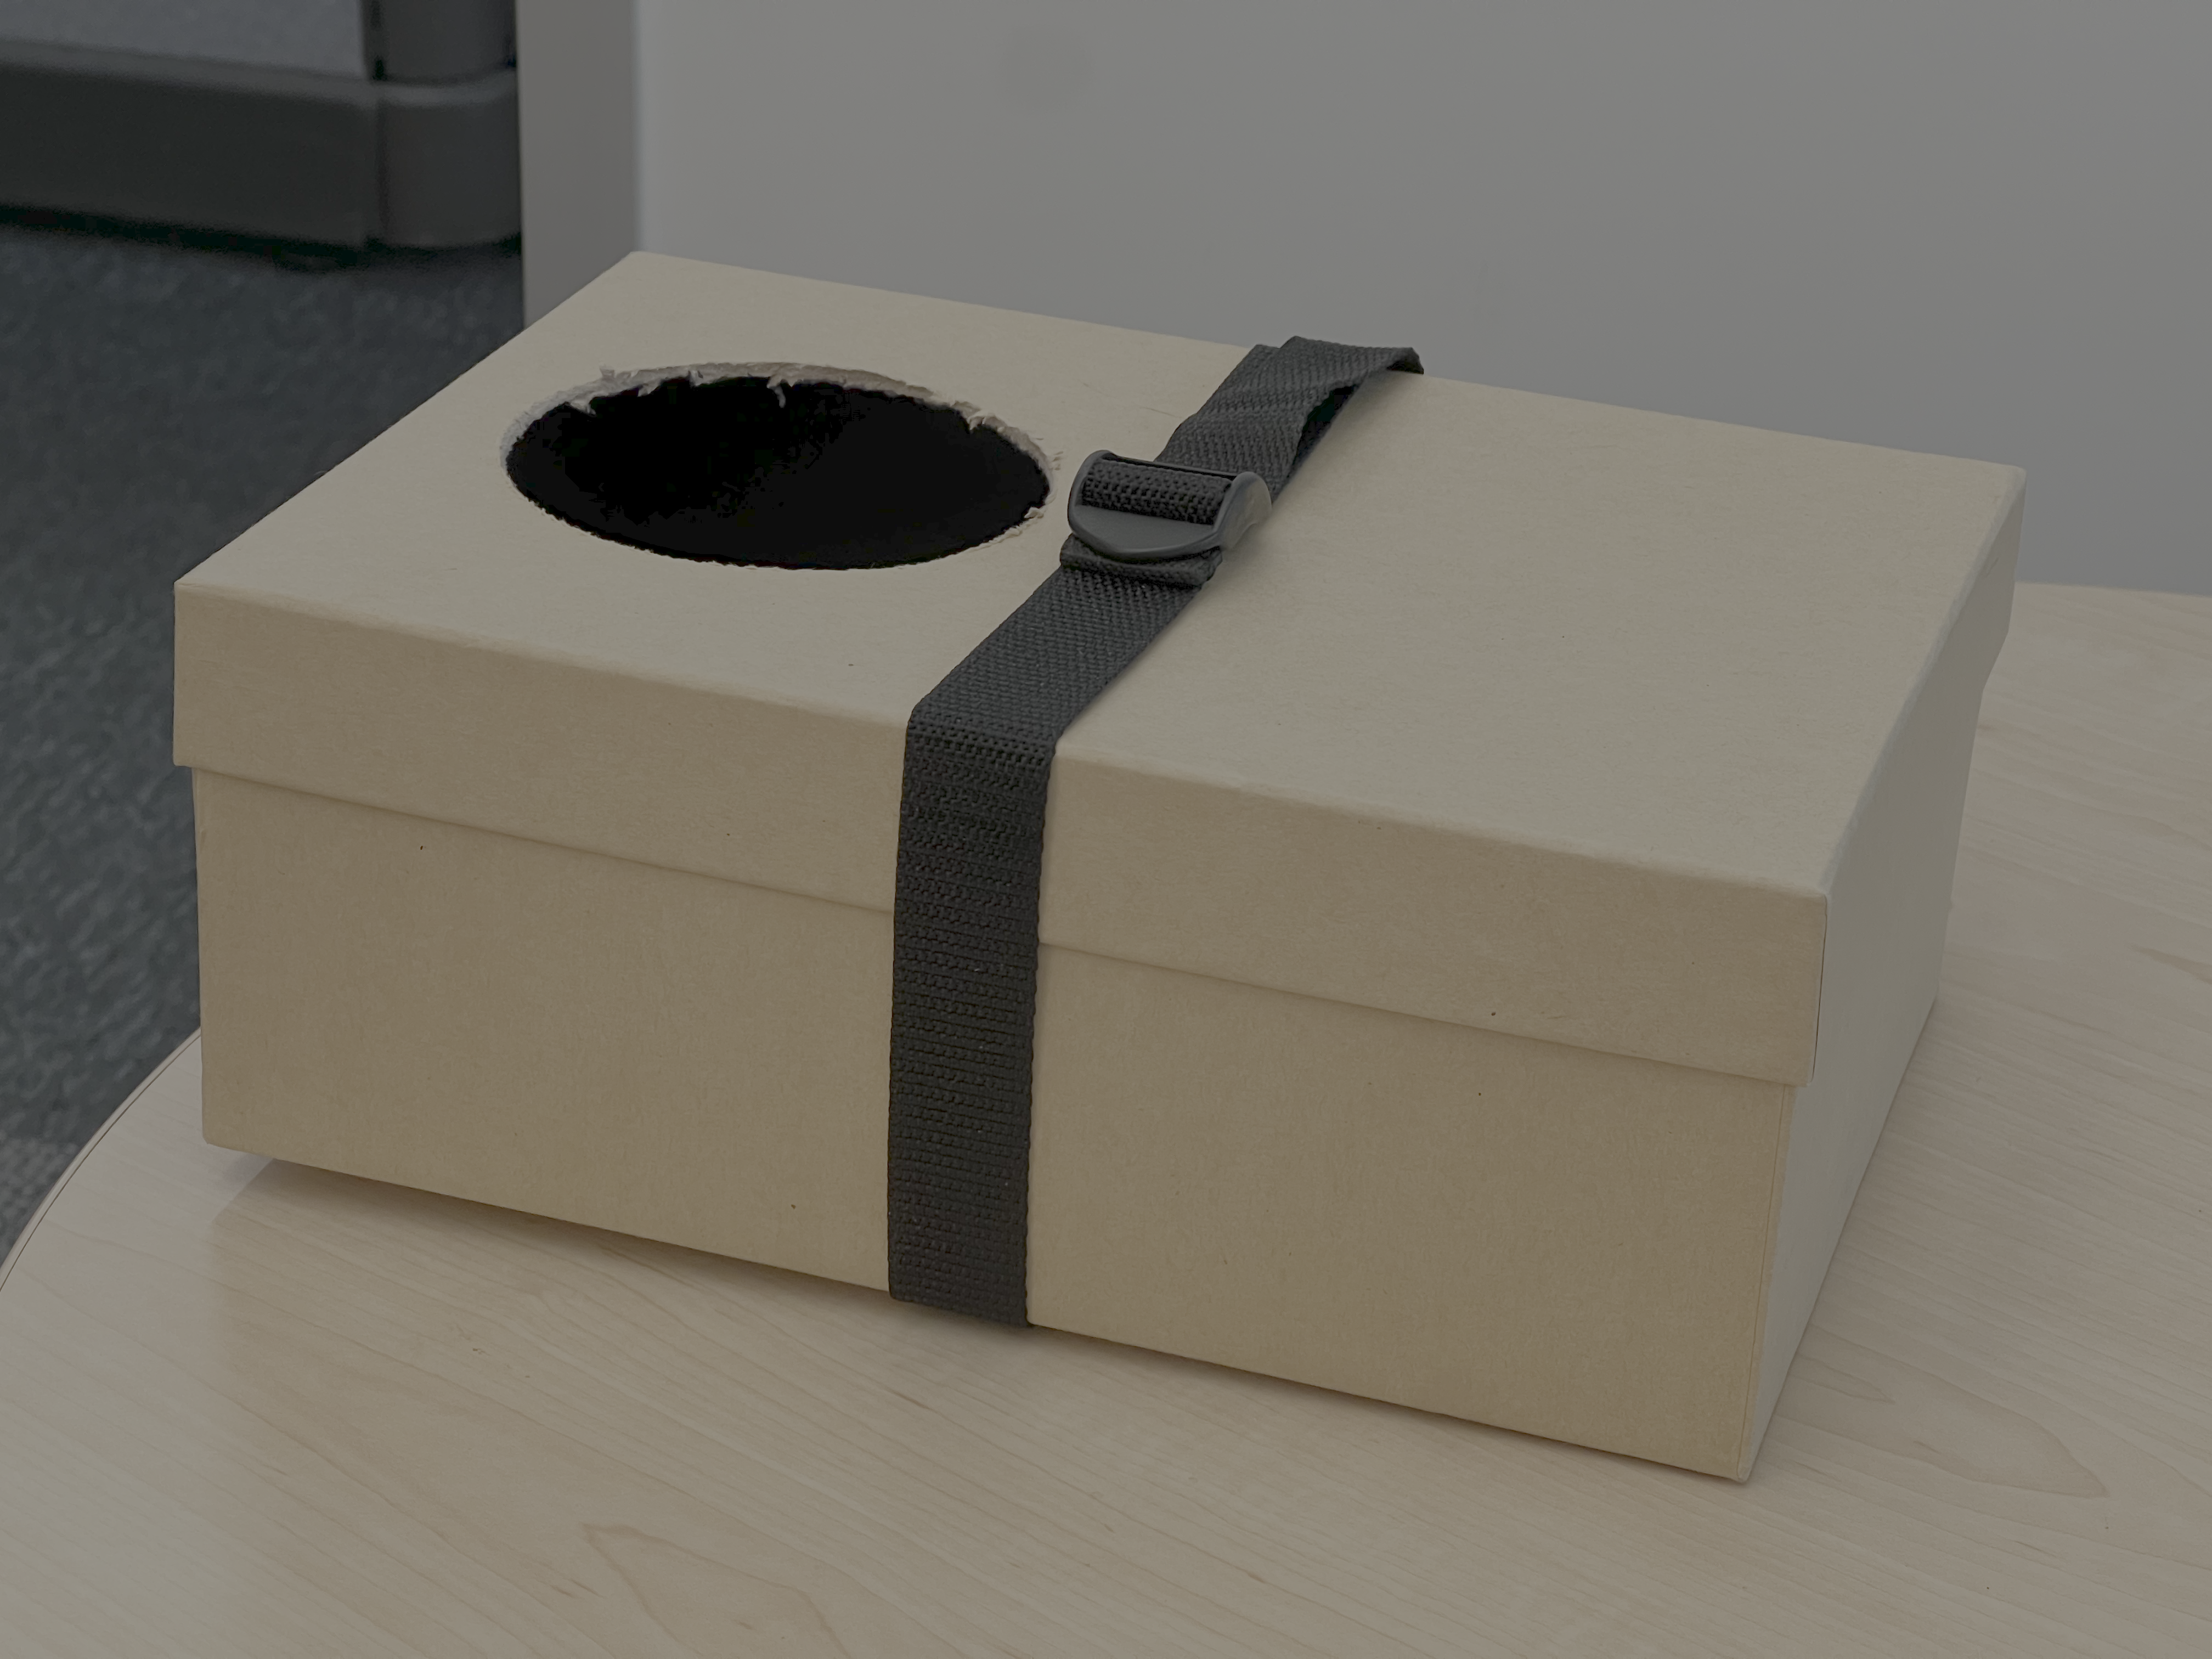
\includegraphics[width=1\linewidth]{figures/IMG_3915.png}
	\end{frame}
	\begin{frame}
		\frametitle{Five Senses, Which is Most Important to You?}
		\begin{columns}
			\begin{column}{.25\linewidth}
				\begin{itemize}
					\item Hearing?
					\item Sight?
					\item Smell?
					\item Taste?
					\item Touch?
				\end{itemize}
			\end{column}
			\begin{column}{.25\linewidth}
				\includegraphics[width=1\linewidth]{figures/4 stick figure high point phase of walk cycle animation tutorial the helpful art teacher.JPG}
			\end{column}
			\begin{column}{.5\linewidth}
				\begin{itemize}
					\item Which of these seems the most valuable to you?
					\item Which would you relinquish last?
				\end{itemize}
			\end{column}
		\end{columns}
	\end{frame}
	\begin{frame}
		\frametitle{Five Senses, Which is Most Important to You?}
		\begin{columns}
			\begin{column}{.375\linewidth}
				Sight
				\includegraphics[width=1\linewidth]{figures/intoxicating_eye_stock_by_taylorinchains-d35yf9n.jpg}
				\begin{itemize}
					\item Centralized
					\item Broad
					\item Passive
					\item Cognitive
				\end{itemize}
			\end{column}
			\begin{column}{.25\linewidth}
				\includegraphics[width=1\linewidth]{figures/4 stick figure high point phase of walk cycle animation tutorial the helpful art teacher.JPG}
			\end{column}
			\begin{column}{.375\linewidth}
				~ % empty, so that it all appears on the next slide
			\end{column}
		\end{columns}
	\end{frame}
	\begin{frame}
		\frametitle{Five Senses, Which is Most Important to You?}
		\begin{columns}
			\begin{column}{.375\linewidth}
				\begin{center}
					Sight
				\end{center}
				\includegraphics[width=1\linewidth]{figures/intoxicating_eye_stock_by_taylorinchains-d35yf9n.jpg}
				\begin{itemize}
					\item Centralized
					\item Broad
					\item Passive
					\item Cognitive
				\end{itemize}
			\end{column}
			\begin{column}{.25\linewidth}
				\includegraphics[width=1\linewidth]{figures/4 stick figure high point phase of walk cycle animation tutorial the helpful art teacher.JPG}
			\end{column}
			\begin{column}{.375\linewidth}
				\begin{center}
					Touch
				\end{center}
				\includegraphics[width=1\linewidth]{figures/wrist-drop.jpg}
				\begin{itemize}
					\item Distributed
					\item Narrow
					\item Interactive
					\item Fundamental
				\end{itemize}
			\end{column}
		\end{columns}
	\end{frame}
	
\section{Define}
	\subsection{Defined: Haptic}
	\begin{frame}
		\frametitle{What is Haptics?}
	  %\setbeamercovered{transparent=20}
		\begin{definition}
			haptic\\ %\textcolor{gray}{| \textipa{/ˈwɛərəbl/} |}\\ % or 'wer\schwa b(\schwa)l 
			\textbf{adjective}\\
			\begin{enumerate}
				\item of or relating to the sense of touch, in particular relating to the perception and manipulation of objects using the senses of touch and proprioception.
			\end{enumerate}
			\textbf{origin}\\
			\begin{enumerate}
				\item late 19th century: from Greek {\em haptikos} {\bf `able to touch or grasp,'} from {\em haptein} {\bf `fasten.'}
			\end{enumerate}
		\end{definition}
	\end{frame}
	\subsection{Defined: (Opt)ics}
	\begin{frame}
		\frametitle{What is (Opt / Informat)ics?}
		\begin{definition}
			optics\\ %\textcolor{gray}{| \textipa{/ˌinfərˈmadiks/} |}\\
			\textbf{plural noun}\\
			\begin{enumerate}
				\item the \underline{scientific study of} sight and the behavior of light, or the properties of transmission and deflection of other forms of radiation.
			\end{enumerate}
		\end{definition}
		\begin{definition}
			in\textbullet for\textbullet mat\textbullet ics\\ %\textcolor{gray}{| \textipa{/ˌinfərˈmadiks/} |}\\
			\textbf{plural noun}\\
			\begin{enumerate}
				\item the \underline{science of} processing data for storage and retrieval; informatics science
			\end{enumerate}
		\end{definition}
	\end{frame}
	\subsection{Defined: Haptics}
	\begin{frame}
		\frametitle{Haptic\underline{s}}
		\begin{definition}
		Haptics
			\begin{itemize}
				\item the science and technology of touch
			\end{itemize}
		\end{definition}
	\end{frame}
	
% 	\subsection{Popularity} % https://trends.google.com/trends/explore?date=today%205-y&geo=US&q=haptics&hl=en-US
% 	\begin{frame}
% 	\frametitle{Google Search Popularity}
% % 	  \setbeamercovered{transparent=20}
% 		\begin{figure}
% 		    \centering
% 		    \begin{tikzpicture}
% 		        \begin{axis}[
% 		            xlabel={Date},
% 		            ylabel={Value},
% 		            title={Popularity of `Haptics' Over Time},
% 		            grid=both,
% 		            date coordinates in = x,
% 		            xticklabel=\month-\year, % https://tikz.dev/pgfplots/reference-tickoptions
% 		            ymajorgrids=true,
% 		            yminorgrids=true,
% 		            %ymin=0, % Adjust y-axis limits if necessary
% 		            %ymax=30,
% 		            width=\linewidth,
% 		            height=6cm,
% 		        ]
% 		        \addplot [thick, no markers] table [x=Week, y=Haptics: (Worldwide), col sep=comma] {multiTimeline.csv}; 
% 		        \end{axis}
% 		    \end{tikzpicture}
% 		    \caption{Time Series Data Visualization}
% 		\end{figure}
% 	\end{frame}
% 	
% 	\begin{frame}
% 	\frametitle{Related Search Topics}
% 		\begin{itemize}
% 			\item Technology (100)
% 			\item Watch (68)
% 			\item Health (63)
% 			\item Wearable computer (59)
% 			\item Sensor (52)
% 			\item Artificial intelligence (46)
% 			\item Data (39)
% 			\item Physical fitness (27)
% 			\item Smartwatch (24)
% 			\item Medicine (23)
% 			\item Sleep (23)
% 		\end{itemize}
% 	\end{frame}

\section{Haptic Exploration}
	\subsection{What's Inside?}
	\begin{frame}
		\frametitle{What's Inside?}
		\centering
		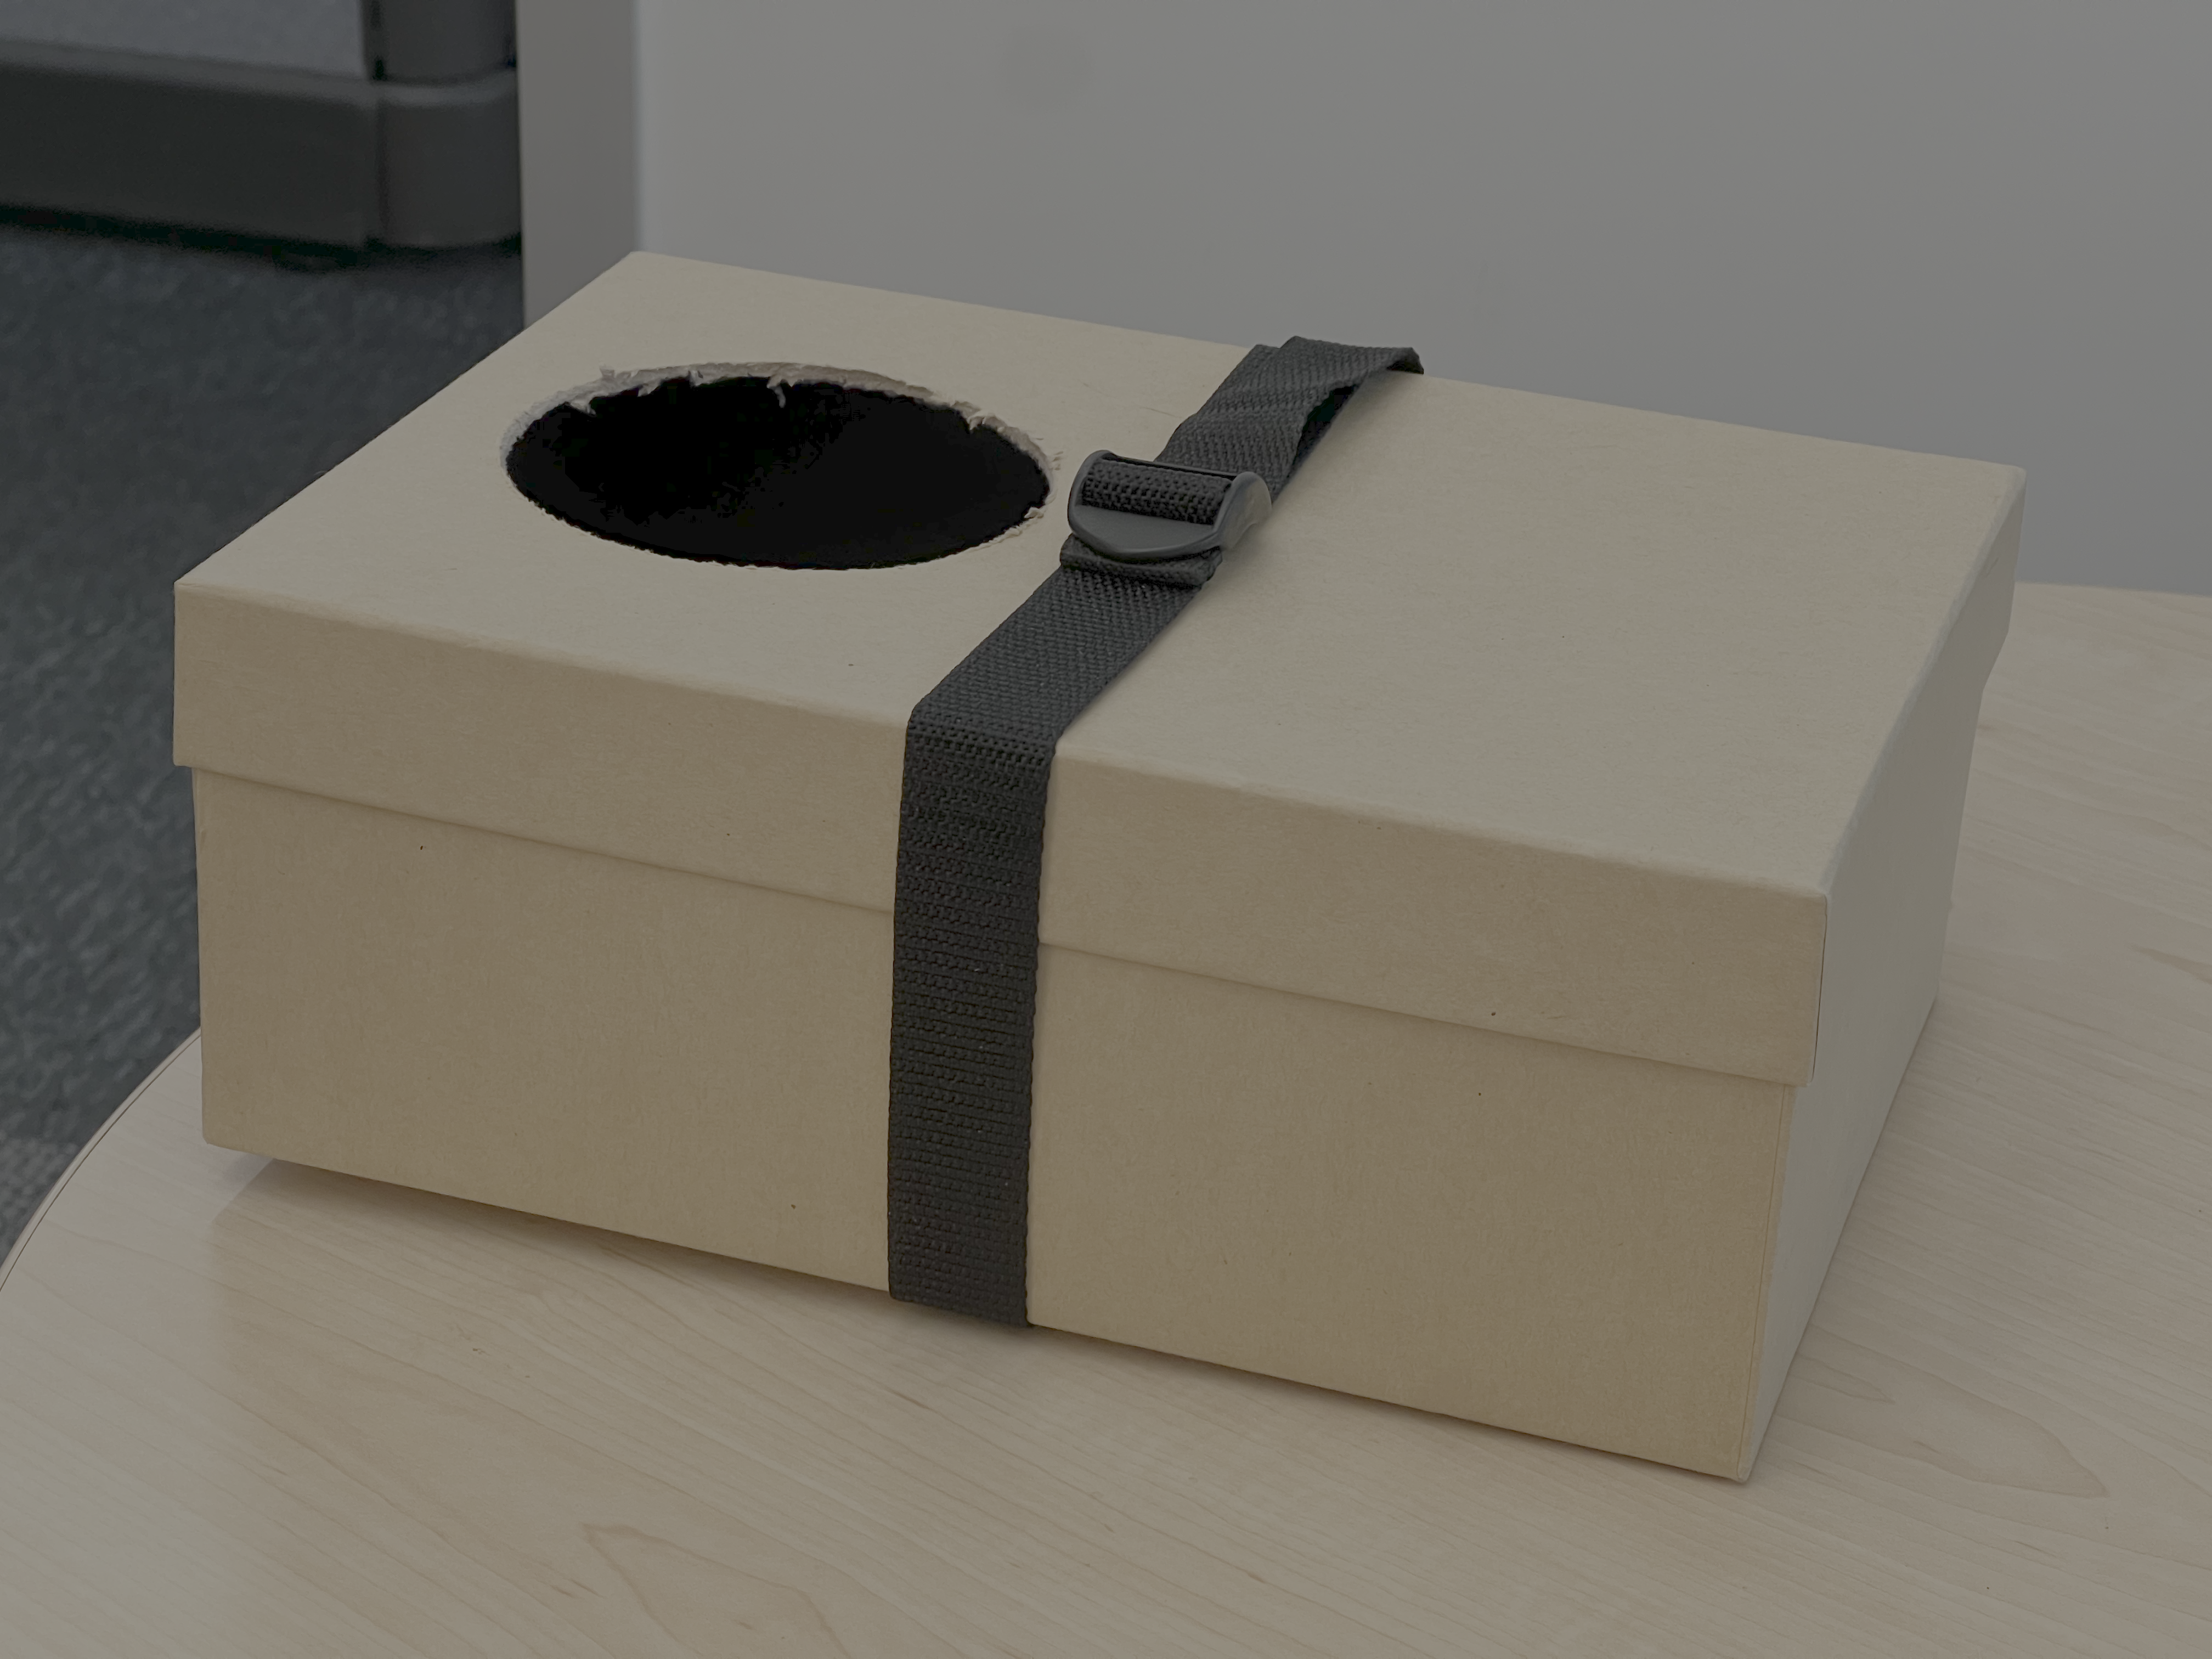
\includegraphics[width=.2\linewidth]{figures/IMG_3915.png}
		%\includegraphics[width=.8\linewidth]{figures/FullSizeRender 2.jpg}
	\end{frame}
	\begin{frame}
		\frametitle{What's Inside?}
		\centering
		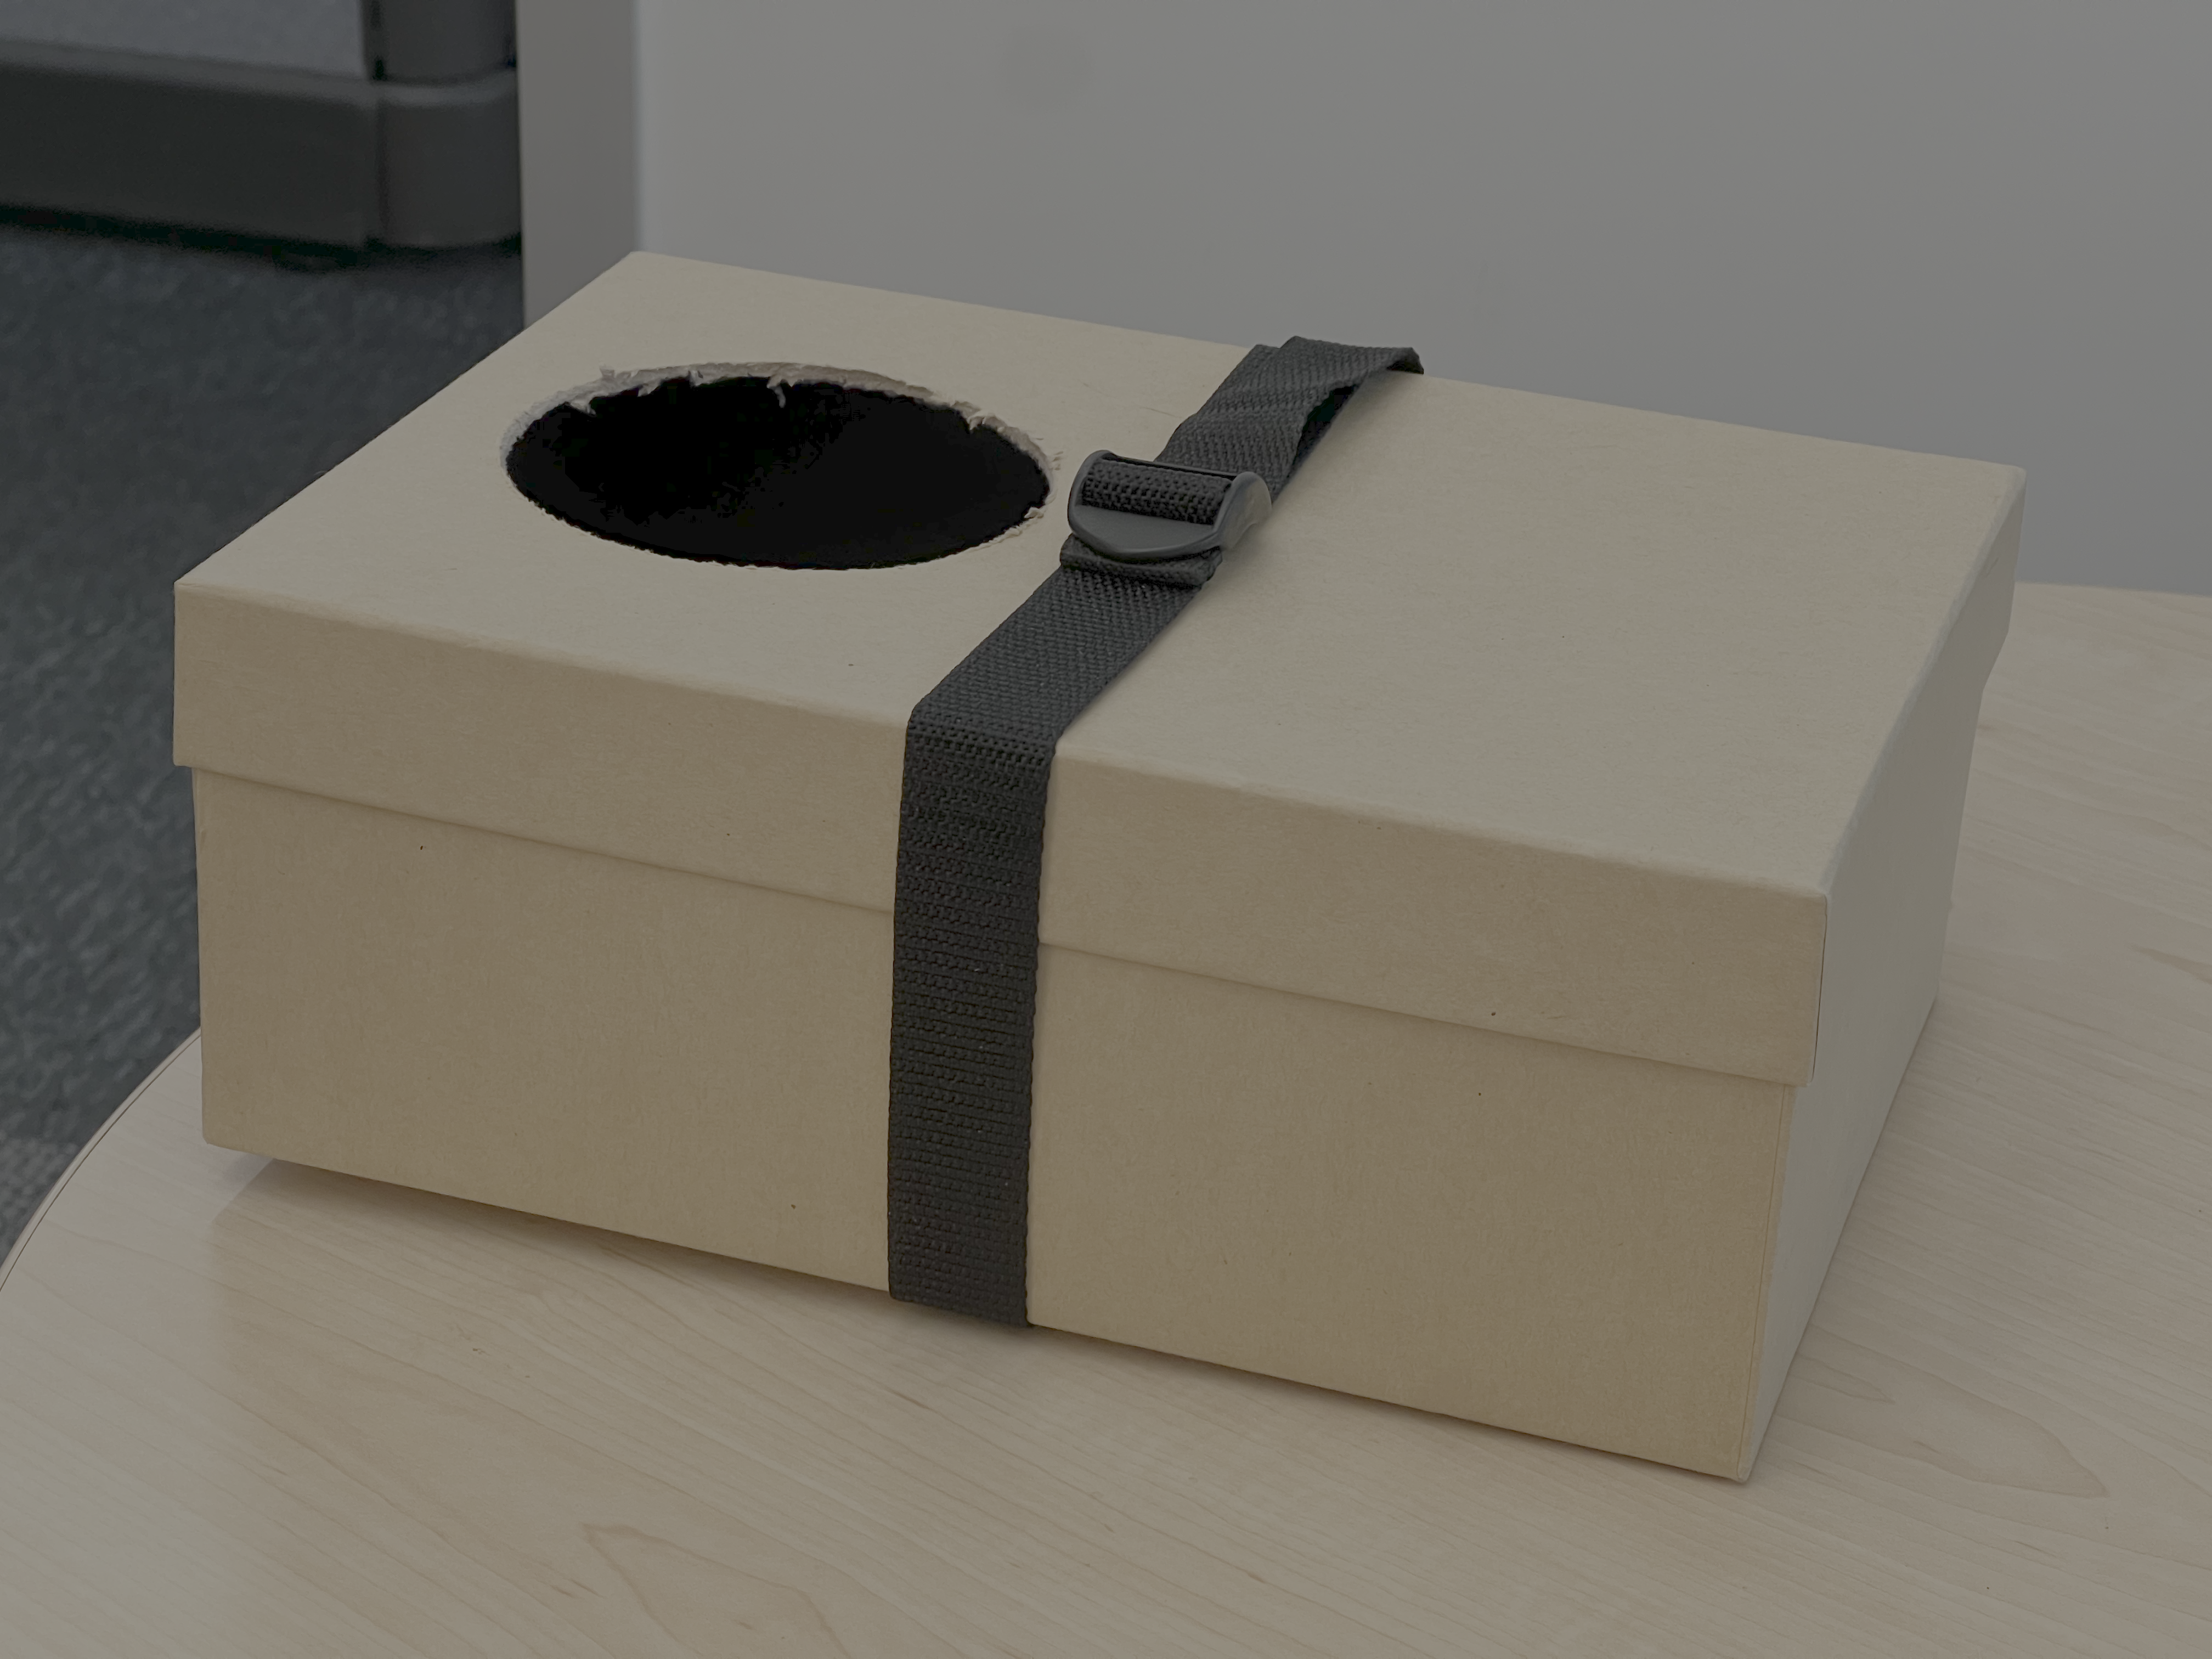
\includegraphics[width=.2\linewidth]{figures/IMG_3915.png}
		\includegraphics[width=.8\linewidth]{figures/FullSizeRender 2.jpg}
	\end{frame}
	\subsection{Exploratory Procedures}
	\begin{frame}
		\frametitle{Exploratory Procedures}
		\centering
		\includegraphics[width=1\linewidth]{figures/Screen Shot 2017-01-30 at 9.31.45 AM.png}
	\end{frame}
	\subsection{Types of Sensing}
	\begin{frame}
		\frametitle{Types of Sensing}
		\centering
		\includegraphics[width=1\linewidth]{figures/Screen Shot 2017-01-30 at 9.33.44 AM.png}
	\end{frame}
	
\section{Haptic Devices}
	\subsection{Tactile and Proprioceptive Devices}
	\begin{frame}
		\frametitle{Tactile and Proprioceptive Devices}
		\centering
		\includegraphics[width=1\linewidth]{figures/Screen Shot 2017-01-30 at 9.40.37 AM.png}
	\end{frame}
	\subsection{Tactile Device Challenges}
	\begin{frame}
		\frametitle{Tactile Device Challenges}
		\begin{columns}
			\begin{column}{.6\linewidth}
			\centering
				\includegraphics[width=1\linewidth]{figures/Screen Shot 2017-01-30 at 9.42.12 AM.png}
				\includegraphics[width=.6\linewidth]{figures/Screen Shot 2017-01-30 at 9.45.52 AM.png}
			\end{column}
			\begin{column}{.4\linewidth}
				%\centering
				\begin{itemize}
					\item Stimulation density needs to be high.
					\item Multimodal sensations are very hard to overlay.
					\item High complexity and weight diminish portability.
					\item Passive touch does not feel real.
					\item Tactile device design is difficult!
				\end{itemize}
			\end{column}
		\end{columns}
	\end{frame}
	\subsection{Kinesthetic Device Challenges}
	\begin{frame}
		\frametitle{Kinesthetic Device Challenges}
		\begin{columns}
			\begin{column}{.6\linewidth}
			\centering
				\includegraphics[width=1\linewidth]{figures/Screen Shot 2017-01-30 at 9.48.31 AM.png}
				\includegraphics[width=.5\linewidth]{figures/Screen Shot 2017-01-30 at 9.49.13 AM.png}
			\end{column}
			\begin{column}{.4\linewidth}
				%\centering
				\begin{itemize}
					\item Competing goals of high stiffness and low mass.
					\item Force feedback feels soft - ``Nerfworld''.
					\item Point based interactions are overly simple.
					\item High quality devices are expensive.
					\item Limited workspace.
					\item Constrained to a desk!
				\end{itemize}
			\end{column}
		\end{columns}
	\end{frame}
	\subsection{Workspace vs Force}
	\begin{frame}
		\frametitle{Workspace vs Force}
		\centering
		\includegraphics[width=1\linewidth]{figures/Screen Shot 2017-01-30 at 9.38.30 AM.png}
	\end{frame}
	\subsection{Haptic Wearables?}
	\begin{frame}
		\frametitle{But what can you do with haptic wearables?}
		\begin{columns}
			\begin{column}{.6\linewidth}
			\begin{itemize}
					\item Vibration (eccentric mass motor or tactor)
					\item Skin stretch
					\item Kinesthetic force
					\item Inertial changes
				\end{itemize}
				\includegraphics[width=.32\linewidth]{figures/HTB1LuJMFVXXXXcqXVXXq6xXFXXXy.jpg}
				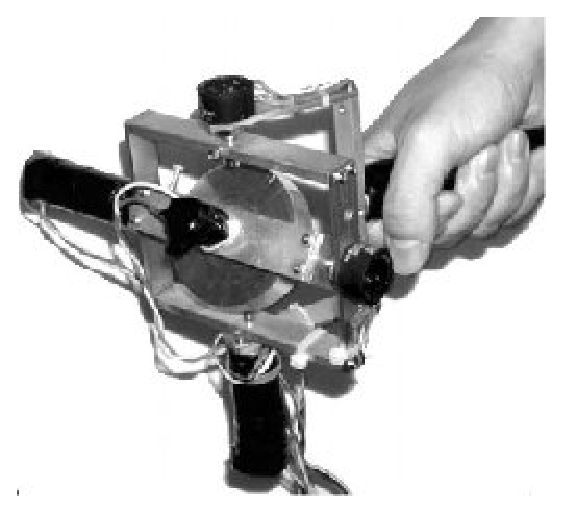
\includegraphics[width=.32\linewidth]{figures/gyro_other.eps}
				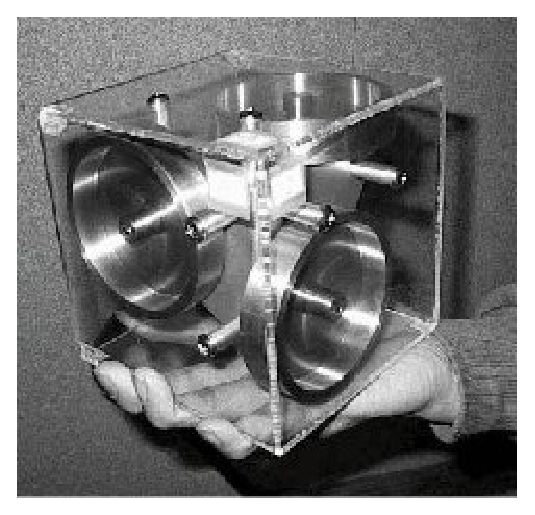
\includegraphics[width=.32\linewidth]{figures/gyro_cube.eps}
			\end{column}
			\begin{column}{.4\linewidth}
				\centering
				\includegraphics[width=1\linewidth]{figures/1714367.jpg}
				\includegraphics[width=1\linewidth]{figures/FuncPrototype_closeup.JPG}
			\end{column}
		\end{columns}
	\end{frame}
\section{Readings}
	\subsection{Thursday}
		\begin{frame}
		\frametitle{Thrusday}
		\footnotesize
			\begin{itemize}
				\item OPTIONAL - Embodied Auxetic Intelligence in a Glove‐Type Wearable Haptic Interface Connecting Humans.pdf
				\item OPTIONAL - FiDTouch - A 3D Wearable Haptic Display for the Finger Pad.pdf
				\item OPTIONAL - Haptics in Teleoperated Medical Interventions -  Force Measurement, Haptic Interfaces and Their Influence on Users Performance.pdf
				\item OPTIONAL - Music Tactalizer - A Wearable Haptic Music Player with Multi-Feature Audio-Tactile Rendering.pdf
				\item OPTIONAL - Predicting the Future with Wearable Technology.pdf
				\item OPTIONAL - The Future of Wearable Technologies and Remote Monitoring in Health Care.pdf
				\item OPTIONAL - Ultralight Soft Wearable Haptic Interface with Shear‐Normal‐Vibration Feedback.pdf
% 				\item {\em TO DISCUSS - Haptic Perception and Its Relation to Action.pdf}
% 				\item {\em TO DISCUSS - Haptic Rendering Introductory Concepts.pdf}
% 				\item {\em TO DISCUSS - The future of wearable technologies.pdf}
			\end{itemize}
		\end{frame}
		\begin{frame}
		\frametitle{Thrusday}
			\begin{itemize}
				\footnotesize
				\item OPTIONAL - Embodied Auxetic Intelligence in a Glove‐Type Wearable Haptic Interface Connecting Humans.pdf
				\item ...
				\item OPTIONAL - Ultralight Soft Wearable Haptic Interface with Shear‐Normal‐Vibration Feedback.pdf
				\normalsize
				\item {\bf TO DISCUSS - Haptic Perception and Its Relation to Action.pdf}
				\item {\bf TO DISCUSS - Haptic Rendering Introductory Concepts.pdf}
				\item {\bf TO DISCUSS - The future of wearable technologies.pdf}
			\end{itemize}
		\end{frame}
\end{document}
